%% 
%% This is file `sample-authordraft.tex',
%% generated with the docstrip utility.
%%
%% The original source files were:
%%
%% samples.dtx  (with options: `authordraft')
%% 
%% IMPORTANT NOTICE:
%% 
%% For the copyright see the source file.
%% 
%% Any modified versions of this file must be renamed
%% with new filenames distinct from sample-authordraft.tex.
%% 
%% For distribution of the original source see the terms
%% for copying and modification in the file samples.dtx.
%% 
%% This generated file may be distributed as long as the
%% original source files, as listed above, are part of the
%% same distribution. (The sources need not necessarily be
%% in the same archive or directory.)
%%
%% The first command in your LaTeX source must be the \documentclass command.
\documentclass[sigconf,authordraft]{acmart}
%\DeclareMathOperator*{\text{maximize}}{Max}

%%
%% \BibTeX command to typeset BibTeX logo in the docs
\AtBeginDocument{%
  \providecommand\BibTeX{{%
    \normalfont B\kern-0.5em{\scshape i\kern-0.25em b}\kern-0.8em\TeX}}}

%% Rights management information.  This information is sent to you
%% when you complete the rights form.  These commands have SAMPLE
%% values in them; it is your responsibility as an author to replace
%% the commands and values with those provided to you when you
%% complete the rights form.
\setcopyright{acmcopyright}
\copyrightyear{2018}
\acmYear{2018}
\acmDOI{10.1145/1122445.1122456}

%% These commands are for a PROCEEDINGS abstract or paper.
\acmConference[Woodstock '18]{Woodstock '18: ACM Symposium on Neural
  Gaze Detection}{June 03--05, 2018}{Woodstock, NY}
\acmBooktitle{Woodstock '18: ACM Symposium on Neural Gaze Detection,
  June 03--05, 2018, Woodstock, NY}
\acmPrice{15.00}
\acmISBN{978-1-4503-9999-9/18/06}


%%
%% Submission ID.
%% Use this when submitting an article to a sponsored event. You'll
%% receive a unique submission ID from the organizers
%% of the event, and this ID should be used as the parameter to this command.
%%\acmSubmissionID{123-A56-BU3}

%%
%% The majority of ACM publications use numbered citations and
%% references.  The command \citestyle{authoryear} switches to the
%% "author year" style.
%%
%% If you are preparing content for an event
%% sponsored by ACM SIGGRAPH, you must use the "author year" style of
%% citations and references.
%% Uncommenting
%% the next command will enable that style. 
%%\citestyle{acmauthoryear} 

%% 
%% end of the preamble, start of the body of the document source. 

\begin{document} 

%% 
%% The "title" command has an optional parameter, 
%% allowing the author to define a "short title" to be used in page headers. 
\title{Optimizing Effectiveness of User Retention with Heterogeneous Sequential Causal Learning} 

%% 
%% The "author" command and its associated commands are used to define
%% the authors and their affiliations.
%% Of note is the shared affiliation of the first two authors, and the
%% "authornote" and "authornotemark" commands
%% used to denote shared contribution to the research.
%\author{Shuyang Du}
%\authornote{Both authors contributed equally to this research.}

%\email{shuyangdu@uber.com}
%\orcid{1234-5678-9012}
%\affiliation{%
%  \institution{Uber}
%  \streetaddress{1455 Market Street}
%  \city{San Francisco}
%  \state{CA}
%}

%\author{Will Y. Zou}
%\authornotemark[1]
%\email{will.zou@uber.com}
%\affiliation{%
%  \institution{Uber}
%  \streetaddress{1455 Market Street}
%  \city{San Francisco}
% \state{CA}
%} 


%% 
%% By default, the full list of authors will be used in the page 
%% headers. Often, this list is too long, and will overlap 
%% other information printed in the page headers. This command allows 
%% the author to define a more concise list 
%% of authors' names for this purpose. 

\renewcommand{\shortauthors}{[tbd]} %Zou and Du, et al. 

%% 
%% The abstract is a short summary of the work to be presented in the 
%% article. 

\begin{abstract} 
User retention and engagement is a key focus for consumer based internet companies. These products make substantial actions to affect users, which lead to real-world changes that boost the volume of active users. The actions requires significant promotional cost with complicated off-set by increase in future revenue. The risk of cost motivates companies to apply churn prediction or regular A/B testing to infer effects of retention treatment. These methods do not capture up-lift across counterfactual outcomes. For predictive models capable of estimating treatment effect, they are also inadequate for optimizing for the balance of cost versus benefit. 

We take an action-result causal perspective to propose a ubiquitous treatment effect optimization framework which learns from past experiments and utilize novel deep learning methods to directly maximize cost effectiveness. Rather than only predicting treatment up-lift, this approach employs a population-wide effectiveness score and significantly improves holistic spend efficiency for entire experiments. The effectiveness of our model surpasses quasi-oracle estimation (r-learner) model and causal forests. We also developed a duality method for the quasi-oracle estimation model, and establish evaluation metrics that reflect the cost-efficiency and real-world business value. Our framework is useful in many product scenarios such as allocating treatment to optimal user selections, and forecast effects of treatments. 

The framework demonstrates superior algorithmic flexibility. Based on the direct optimization algorithm, we develop the top-quantile ranking method to enable optimization with inherent cost constraints, outperforming the baseline method by 15\%. Due to sequential and long-term nature of user retention, we develop a recurrent deep learning model with LSTMs to form a sequential causal learning model. When applied on user context states across 11 weeks, we observe 28\% improvement upon the direct optimization ranking method. 

%Finally, we propose evaluation metrics to captures real-world business value and cost efficiency of different methods. These methods have been deployed to production and is currently live in multiple cities all over the world. 

% weighting labels in cohorts to compute expected difference in cost and gain. With such, an overall effectiveness objective can be computed. Gradient methods are used to find minima of the objective function by changing parameters in the model.  
%We also develop an evaluation metric that captures the real-world business value of different methods and use this to evaluate various approaches on our large-scale experiment data set both offline and online. Our algorithm (approach 2) is significantly better than random explore benchmark and existing estimators (approach 1) in both offline and online test. This method has been deployed to production and is currently live in multiple cities all over the world. 
\end{abstract} 

%%
%% The code below is generated by the tool at http://dl.acm.org/ccs.cfm.
%% Please copy and paste the code instead of the example below.
%%
%\begin{CCSXML}
%<ccs2012>
% <concept>
%  <concept_id>10010520.10010553.10010562</concept_id>
%  <concept_desc>Computer systems organization~Embedded systems</concept_desc>
%  <concept_significance>500</concept_significance>
% </concept>
% <concept>
%  <concept_id>10010520.10010575.10010755</concept_id>
%  <concept_desc>Computer systems organization~Redundancy</concept_desc>
%  <concept_significance>300</concept_significance>
% </concept>
% <concept>
%  <concept_id>10010520.10010553.10010554</concept_id>
%  <concept_desc>Computer systems organization~Robotics</concept_desc>
%  <concept_significance>100</concept_significance>
% </concept>
 %<concept>
%  <concept_id>10003033.10003083.10003095</concept_id>
%  <concept_desc>Networks~Network reliability</concept_desc>
%  <concept_significance>100</concept_significance>
% </concept>
%</ccs2012>
%\end{CCSXML}

%\ccsdesc[500]{Computer systems organization~Embedded systems}
%\ccsdesc[300]{Computer systems organization~Redundancy}
%\ccsdesc{Computer systems organization~Robotics}
%\ccsdesc[100]{Networks~Network reliability}

%%
%% Keywords. The author(s) should pick words that accurately describe
%% the work being presented. Separate the keywords with commas.
\keywords{Causal Inference; Heterogeneous Treatment Effect; Optimization; Deep Learning; Neural Networks; User Engagement; User Retention} 

%% A "teaser" image appears between the author and affiliation
%% information and the body of the document, and typically spans the
%% page.
%\begin{teaserfigure}
%  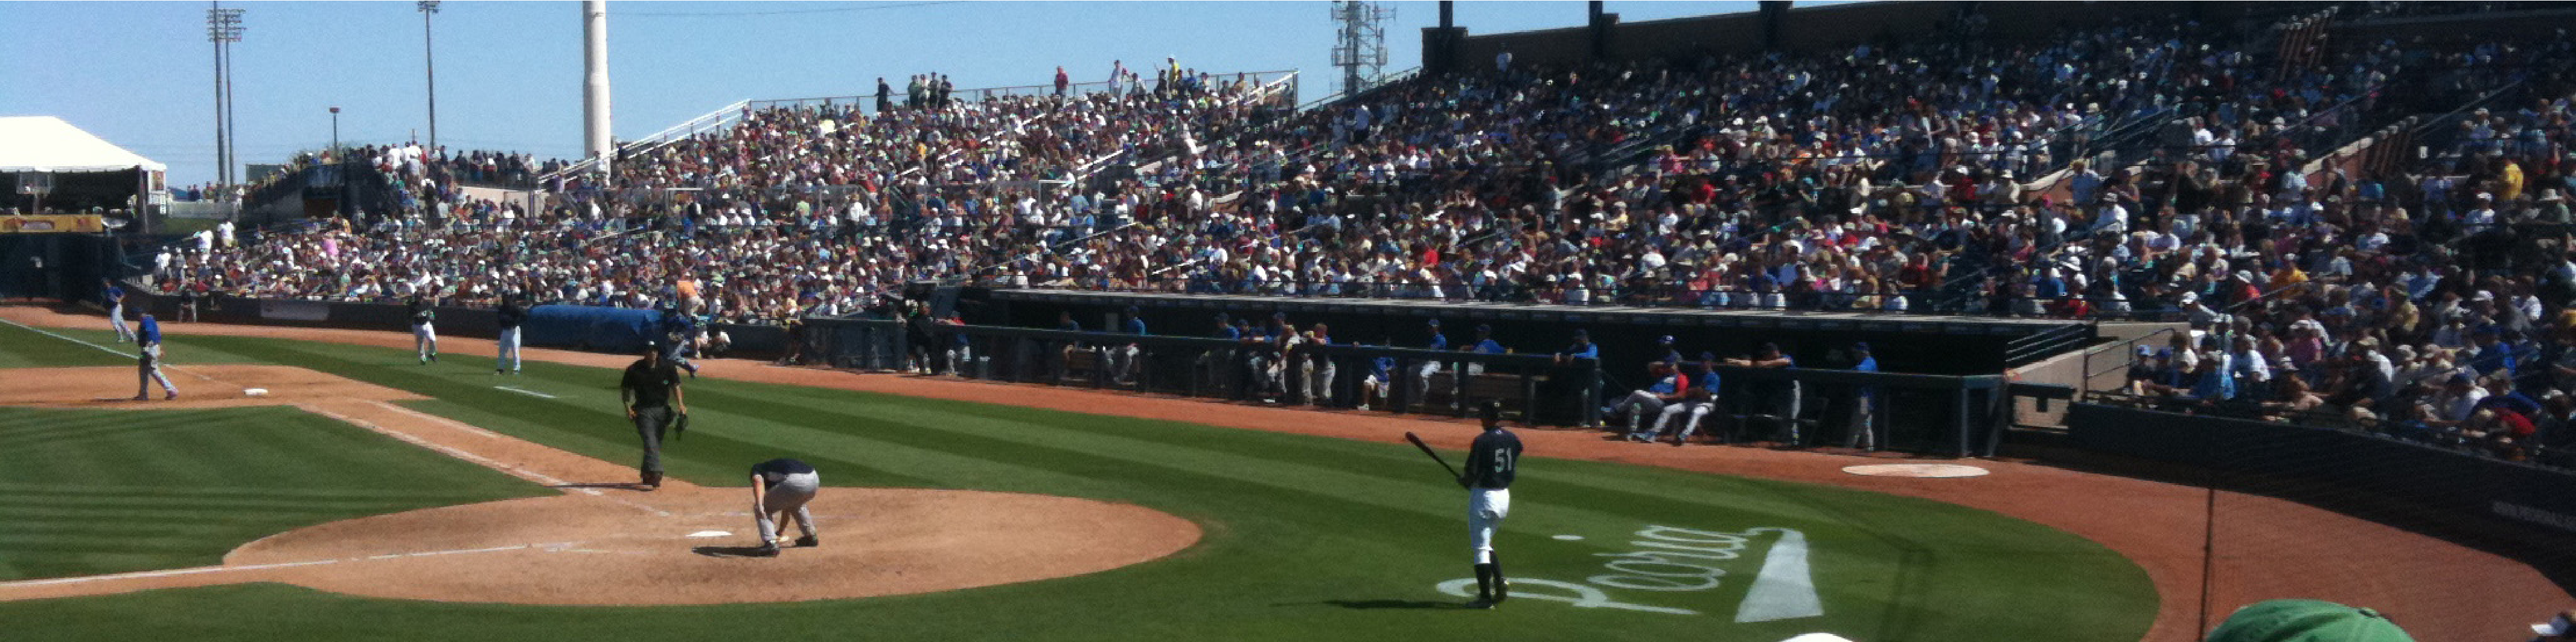
\includegraphics[width=\textwidth]{sampleteaser}
%  \caption{Seattle Mariners at Spring Training, 2010.}
%  \Description{Enjoying the baseball game from the third-base 
% seats. Ichiro Suzuki preparing to bat.} 
%  \label{fig:teaser} 
%\end{teaserfigure} 

%% 
%% This command processes the author and affiliation and title 
%% information and builds the first part of the formatted document. 

\maketitle 

\section{Introduction}
\label{sec:intro} 
Improving user retention and preventing user churn have become an important focus for many internet companies as the market matures and the cost of acquiring new users rises. In addition to the natural friction, experiencing poor service is one of the main driving factors behind user churn. In different industries, companies provide different services, examples include accommodation (Airbnb), ride-sharing (Uber, Lyft), and e-commerce (Amazon, Ebay).

As suggested in previous research [1] from Uber, providing a user with a promotion without explicit apology after an unsatisfactory trip experience will have a positive treatment effect on future billings. This is consistent with the finding in [2] where researchers conducted a similar experiment on Via (a ride-sharing company in NYC). However previous research and common practice relies on non-causal churn prediction or heuristics based on frustrating experiences for promo decisions instead of directly optimizing for users' promotional treatment effects. 

The goal of our work is to provide a framework to directly optimize for the overall effectiveness of treatments. Partially, this includes maximizing the treatment effect of promotions on user retention. This framework has the combined effect of minimizing cost, reduce user churn (especially caused by experiencing an unsatisfactory service), and creating uplift in desired metrics. Compared to existing work on user promotions and heterogeneous treatment effect estimation, novel contributions of this paper are: 

\begin{itemize}

\item\textbf{Framework for Heterogeneous Treatment Effect for Business Decisions} - A common approach for promotion decisions relies on regular predictions, redemptions or heuristics which are tied to specific scenario and require rich background context. In this paper we propose a general framework that directly optimizes the promotional heterogeneous treatment effect and could be applied to various business use cases with minimum change. This approach can be evaluated effectively and give guidance to decisions. 

\item \textbf{Direct Optimization of Effectiveness for Aggregated Treatment Effect} - Most research studies focus on treatment effect of one single value and treat the cost of that treatment as fixed. However, in real-world applications it’s necessary to estimate treatment effect on the cost, i.e. apply the efficiency ratio of $\delta$cost/$\delta$value when making the resource allocation decision. Similar to search ranking versus point estimates of Click Through Rate (CTR), our objective is to maximize aggregated treatment effect instead of having a perfect individual treatment effect and thus we could achieve better performance. We propose a novel algorithm to solve this treatment effect ranking problem. 

\item \textbf{Deep Learning and with Quantile Constraints} - With algorithmic flexibility of our proposal, we apply deep learning algorithms to be able to deal with sophisticated objective functions which addresses cost vs gain. In turn, algorithms are proposed with deep learning to focus on user quantiles to flexibly deal with budget constraints. 

\item \textbf{Recurrent Sequential Causal Learning} - Cadence or sequences of treatments can change user behavior in sophisticated ways, and affect users in the long term. A sequential causal learning algorithm to consider actions across many treatment periods to learn their combined effect, with step-wise changes in user states. Both algorithms are shown to out-perform prior art including our proposal. 

%\item \textbf{Empirical Evaluation Method} - A common difficulty in comparing the accuracy of heterogeneous treatment effect estimators on real data is that we do not have access to the ground truth. The alternative adopted by some research is the uplift curve [16]. In this paper we propose the “cost curve”, a metric designed for the efficiency ratio case above and is consistent with live performance. 

\end{itemize} 

The structure of this paper is as follows: in Section~\ref{sec:related_work}, we will cover related work in optimization of treatment effect. In Section~\ref{sec:algorithms}, we make the problem and introducing effectiveness measures (i.e. cost-curve), and our modeling approaches for treatment effect optimization. In Section~\ref{sec:empirical_results}, we will offer a technical description of experimentation, results, and comparison comparison across models and real-world performance from the product we already launched. Finally we briefly cover future research steps. 

%%propose an evaluation metric to captures real-world business value and cost efficiency of different methods. 

\section{Background} 
\label{sec:related_work} 
Methods for user retention have been widely studied. Two recent studies by Halperin et al. [1] and Cohen et al. [2]  look into the effect of apology promotions when the user's trust is compromised. Andrews et al. [19] studied factors that affect coupon redemption. Hanna et al. [20] and Manzoor and Akoglu [21] investigated factors that influence redemption of time limited promotions. These studies focus on redemption or exploratory average treatment effect and do not explore the promotional optimization. 

Optimization of user engagement is related to~\cite{rubin1974estimating} with a framework for studying treatment effects. In this framework, user instances are treated with an action, and when the outcome is observed it is used in model fitting. One significant area is application of statistical methods such as~\cite{kunzel2017meta} that decomposes the learning algorithm into composite models with \emph{meta-learners}. The study of \emph{meta-learners} have developed to a variety of models, with support from propensity weighting, causal inference and statistics. Another area is application of decision trees and random forests, for instance, uplift tree\cite{rzepakowski2012decision}, causal tree and random forests~\cite{wager2017estimation} , boosting~\cite{powers2017some} are powerful components to build causal inference models. Recently, a widely-adopted framework for learning heterogeneous treatment effect is the work of quasi-oracle estimation by~\cite{nie2017quasi}, and proven to be effective when estimating the up-lift effect in a single outcome. In this work we propose a set of algorithms which not only able to predict effect of treatment, but also combine multiple outcomes into real-world effectiveness measures that can be optimized directly using deep learning. 

Many methods consider the \emph{Individual Treatment Effect (ITE)}, which is the treatment effect predicted by the model per individual user. This can be estimated through generalization if the user context is given and models are commonly based on regression of treatment effects~\cite{kunzel2017meta}. Another measurement is \emph{Average Treatment Effect (ATE)}, this is measured by the statistical quantities of the user population, with prior selection, constraint enforced by the model. Quantities related to retention are up-lift in transactions per user, the promotion cost per user. 

\subsection{Problem Statement: Treatment Effect} 
We formalize our problem with the potential outcomes framework (Neyman, 1923; Rubin, 1974~\cite{rubin1974estimating}) consistent with prior work~\cite{nie2017quasi}. In the user retention case, users are $n$ independent and identically distributed examples indexed by $i$, where $\mathbf{X}^{(i)}$ denotes per-sample features for user $i$ while $\mathbf{X}$ is the entire dataset, $Y_1^{(i)}$ is the observed outcome if treated, and $Y_0^{(i)}$ is observed outcome if not treated. $T^{(i)}$ is the treatment assignment and is binary for a particular treatment type, i.e. $T^{(i)} \in \{0, 1\}$. 

We assume the treatment assignment is unconfounded, i.e., the outcome pair is independent of treatment label given the user features, or treatment assignment is as good as random once we control for the features  (Rosenbaum and Rubin, 1983): $\{Y_0, Y_1\} \perp T_i|\mathbf{X}_i$. This is the assumption we make on all causal models we explore in the paper. The treatment propensity, the probability of a user receiving treatment as $e(\mathbf{x}^{(i)}) = P (T = 1  | \mathbf{X}^{(i)} = \mathbf{x}^{(i)})$. 

With historical experiments, outcomes are observed given the treatment assignments. With each user we would have only observed one outcome per treatment. This historical data can be used to fit a model. For treatment effect estimation, we seek to estimate, with the fitted model, the treatment effect function given that we observe user features $X$: 

\begin{align} 
\tau^*(\mathbf{x}) = E(Y_1 - Y_0 | \mathbf{X} = \mathbf{x})
\end{align} 
%Or the conditional individual treatment effect: 
%\begin{align} 
%\tau^*(\mathbf{x}^{(i)}) = E(Y_1^{(i)} - Y_0^{(i)} | \mathbf{X}^{(i)} = \mathbf{x}^{(i)}) 
%\end{align} 

\subsection{Quasi-oracle Estimation} 
Closely related to our work, we briefly review of the quasi-oracle estimation algorithm~\cite{nie2017quasi} for heterogeneous treatment effects, also known as \emph{`r-learner'} as a \emph{meta-learner}. The quasi-oracle estimation algorithm is a two-step algorithm for observational studies of treatment effects. The marginal effects and treatment propensities are first evaluated in order to form an objective function that isolates the causal component of the signal. Then the algorithm optimizes for the up-lift or causal component using regression or other objective functions. 

Concretely, the conditional mean of outcomes give user features are $\mu^{*}_T(\mathbf{x}) = E(Y_T | \mathbf{X} = \mathbf{x})$, thus expected value of outcome from the model is $E(Y_T^{(i)} | \mathbf{X}^{(i)}) = E(Y_0^{(i)} | \mathbf{X}^{(i)}) + T^{(i)} E(Y_1^{(i)} - Y_0^{(i)} | \mathbf{X}^{(i)}) = \mu^*_0(\mathbf{X}^{(i)}) + T^{(i)}\tau^*(\mathbf{X}^{(i)})$. The expected value of the error across data and expected value of Y is zero given unconfoundedness assumption: 

\begin{align} 
E(\epsilon(T^{(i)}) | \mathbf{X}^{(i)}, T^{(i)}) = 0
\end{align} 

Replacing $E(Y_T^{(i)})$ in the error, and substitute the condition mean outcome: $\epsilon(T^{(i)}) = Y_T^{(i)} - E(Y_T^{(i)}) = Y_T^{(i)} - (\mu^*_0(\mathbf{X}^{(i)}) + T^{(i)}\tau^*(\mathbf{X}^{(i)}))$; $m^*(\mathbf{x}^{(i)}) = E(Y^{(i)} | \mathbf{X}^{(i)} = \mathbf{x}^{(i)})$, we arrive at the decomposition: 

%\begin{align}
%\epsilon(T^{(i)}) &= Y_T^{(i)} - E(Y_T^{(i)}) = Y_T^{(i)} - (\mu^*_0(\mathbf{X}^{(i)}) + T^{(i)}\tau^*(\mathbf{X}^{(i)}))
%\end{align}
%\begin{align}
%m^*(\mathbf{x}^{(i)}) &= E(Y^{(i)} | \mathbf{X}^{(i)} = \mathbf{x}^{(i)})
%\end{align}


\begin{align}
\label{eq:quasi_oracle_balance}
Y^{(i)} - m^*(\mathbf{X}^{(i)}) = (T^{(i)} - e^*(\mathbf{X}^{(i)})\tau^*(\mathbf{X}^{(i)}) + \epsilon
\end{align}

An equation that balances difference between outcome with a `mean' model with the conditional average treatment effect function. In a simple formulation of the quasi-oracle estimation algorithm a regression is used to fit the $m^*$ and $e^*$ models as the first step. The prediction result of the regression is then used to determine the regression target of $\tau^*$ model, which is then fitted also as a regression. After the learning, $\tau^*$ function can be used to estimate the treatment effect given user with feature $\mathbf{X}^{(i)}$. 

%Here we consider R-learner and Causal Forest as the treatment effect estimator. R-learner is a synthetic control fashion two-step algorithm that estimates the marginal effect and then isolates the causal component. Causal Forest is a matching fashion tree-based ensemble algorithm that directly estimates the treatment effect under each tree leaf. Generally we can train above models and have cardinal predictions $\hat{\tau}(x_i)$ for value (retention) and cost. 

%Data science efforts have also surveyed effective models and explore multiple treatments using A/B testing~\cite{}. 
%Due to significant interest to develop flexible and effective algorithms, the work is sub-divided into area

%These advances include methods based on Lasso [22], meta learners [9], recursive partitioning [5], neural networks [7], and most recently quasi-oracle estimation [3]. A recent survey by Dorie et al. [8] used  simulations and empirical datasets to show that these estimators can achieve good heterogeneous treatment effect estimation. However, they didn’t consider the special case of a constraint optimization problem where both cost and value are treatment effects. 

%Optimization. Our problem could be formed as a Knapsack problem [17]. Due to the large number of items and the small scale of the value and cost for each item, greedy approximation can achieve decent results [18]. That said, this work can also use some other optimization algorithm such as SGD [12] and Adam optimizer [13]. These two algorithms are implemented in TensorFlow [15] and provide the foundation for training of our methodology. 

\section{Algorithms} 
\label{sec:algorithms} 
\subsection{Problem Statement: Balanced Effectiveness} 
The quasi-oracle estimation algorithm, among other meta-learner algorithms~\cite{kunzel2017meta}, is efficient at estimating treatment effects of users. However, treatment commonly leads to changes in multiple outcomes. For instance, a retention promotion could lead to the user coming back to the platform and make more transactions, it also lead to a variable increase in cost including the retention cost, offset by the user's positive contributions, so eventual goal is to maximize gains and minimize costs. Many problems in causal learning and reinforcement learning domain trades off the cost of action taking, with the reward obtained by those actions[ref required]. Thus cost effectiveness is a key theme in data science applications of causal inference. In this paper, we propose that causal inference paradigm to maximize cost effectiveness of heterogeneous treatments. 

Concretely, we refresh the problem statement. Instead of estimating the treatment effect function $\tau^*(\mathbf{x}) = E(Y_1 - Y_0 | \mathbf{X} = \mathbf{x})$, we propose to solve the following two problems. The first is a constrained optimization problem for maximizing gain (minimizing negative gain) subject to a budget constraint: 
\begin{align} 
\label{eq:pstatement_constrained} 
\begin{split}
  \text{minimize} \quad -&\sum_{i=1}^n\tau^{*r}(\mathbf{x}^{(i)})z_i \\ 
  \text{subject to} \quad &\sum_{i=1}^n\tau^{*c}(\mathbf{x}^{(i)})z_i \leq B \\
	&\ 0\leq z_i \leq 1 
\end{split}
\end{align} 
With constant $B>0$.  
The second is an unconstrained optimization problem where we minimize the cost per unit of gain: 
\begin{align} 
\label{eq:pstatement_unconstrained_opt} 
\text{minimize} \quad \frac{\overline{\tau}^{*c}(\mathbf{x})}{\overline{\tau}^{*r}(\mathbf{x})} 
\end{align} 

In these optimization problems, we represent treatment effects in terms of retention gains $\tau^{*r}(\mathbf{x}^{(i)}) = E(Y_1^r - Y_0^r | \mathbf{X}^{(i)} = \mathbf{x}^{(i)})$ and cost $\tau^{*c}(\mathbf{x}^{(i)}) = E(Y_1^c - Y_0^c | \mathbf{X}^{(i)} = \mathbf{x}^{(i)})$. Also the overlined $\overline{\tau}^{*r}(\mathbf{x}) = E(Y_1^r - Y_0^r | \mathbf{X} = \{\mathbf{x}^{(i)}\})$ and $\overline{\tau}^{*c}(\mathbf{x}) = E(Y_1^c - Y_0^c | \mathbf{X} = \{\mathbf{x}^{(i)}\})$ are expectations further across the entire population of users. It is important to note these values are part of the optimization objective, but are not strictly a regression function, and we optimize for the exact problems stated above. 

\subsection{Duality R-learner: Duality Method with Quasi-oracle Estimation} 
We describe the duality method with Lagrangian multipliers. This method can be used to solve the constrained optimization in Equation~\ref{eq:pstatement_constrained}, i.e. to maximize the total treatment effect on user retention with a given promotion cost budget. 

First, we assume the CATE functions are fixed, so we solve Problem~\ref{eq:pstatement_constrained} assuming $\tau^{*r}(\mathbf{x}^{(i)})$ and $\tau^{*c}(\mathbf{x}^{(i)})$ are given. Applying one Lagrangian multiplier, the Lagrangian for Problem~\ref{eq:pstatement_constrained}: 

\begin{equation} 
  \label{eq:lagrangian} 
  L(\mathbf{z}, \lambda)=-\sum_{i=1}^n\tau^{*r}(\mathbf{x}^{(i)})z_i + \lambda (\sum_{i=1}^n\tau^{*c}(\mathbf{x}^{(i)})z_i - B) \\ 
\end{equation} 

The optimization in Problem~\ref{eq:pstatement_constrained} can then be rewritten in its Dual form to maximize the Lagrangian dual function $g = \inf_{x\in\emph{D}}L(\mathbf{z}, \lambda)$: 

\begin{align} 
\label{eq:duality_problem} 
\begin{split}
  \max\limits_{\lambda} \inf_{\mathbf{z} \in \emph{D}} \quad L(\mathbf{z}, \lambda) \quad
  \text{subject to} \ 0\leq z_i \leq 1, \lambda \geq 0 \\
\end{split}
\end{align} 

We need to address the caveats for solving the problem with duality, and determine whether the dual problem has the same minimum with original problem. 

\begin{itemize} 
\item If $p(\mathbf{z}, \lambda) = -\sum_{i=1}^n\tau^{*r}(\mathbf{x}^{(i)})z_i$, we know, for the optimal values of the two problems, $p^* \leq g^*$ holds from convex optimization. Equality $p^* = g^*$ holds if $p$, $g$ are convex, and the \emph{Slater constraint qualification} holds, which requires the problem to be strictly feasible. 
\item For any values of $B > 0$, if we consider very small values of some $z_i$, the strict inequality $\sum_{i=1}^n\tau^{*c}(\mathbf{x}^{(i)})z_i < B$ can always hold. Further, $B$ is usually large for a retention campaign. Thus Slater qualifications hold. 
\end{itemize} 

From the analysis above, Problem~\ref{eq:pstatement_constrained} and its dual problem~\ref{eq:duality_problem} are equivalent, and we can solve Problem~\ref{eq:duality_problem} by iteratively optimizing with respect to $\mathbf{z}, \lambda$.  

\textbf{Optimize $\mathbf{z_i}$:} Keeping $\lambda, \mathbf{w}$ fixed, as $\lambda$ and $\ B$ are constants, Problem~\ref{eq:duality_problem} becomes: 
%\begin{equation} 
%  \label{eq:lagrangian_reduced}
%  max \ g=\sum_{i=1}^n\tau^r(x_i)z_i - \lambda\sum_{i=1}^n\tau^c(x_i)z_i
%\end{equation}
%And $g$ could be rewritten as Eq. (\ref{eq:lagrangian_reduced_2}). 
\begin{equation} 
\begin{split}
  \label{eq:lagrangian_reduced}
  \text{maximize}\quad \sum_{i=1}^nz_i s_i \\
  \text{subject to} \quad 0\leq z_i \leq 1
\end{split}
\end{equation} 
Where we define the \emph{effectiveness score} $s_i = \tau^{*r}(\mathbf{x}^{(i)})-\lambda\tau^{*c}(\mathbf{x}^{(i)})$. This optimization problem has a straightforward solution: assign the multiplier $z_i = 1$ when the ranking score $s_i \geq 0$ and assign $z_i = 0$ when ranking score $s_i < 0$. 

\textbf{Optimize $\lambda$:} Take the derivative of $L$ w.r.t $\lambda$, we have its gradient $\frac{\partial g}{\partial \lambda}=B-\sum_{i=1}^n\tau^{*c}(\mathbf{x}^{(i)})z_i$ and update $\lambda$ by Eq. (\ref{eq:update_lambda}) where $\alpha$ is the learning rate. 
\begin{equation}
  \label{eq:update_lambda}
  \lambda\rightarrow \lambda + \alpha(B-\sum_{i=1}^n\tau^{*c}(\mathbf{x}^{(i)}))
\end{equation}
Based on the two steps above, we can iteratively solve for both $z_i$ and $\lambda$ \cite{bertsekas1999nonlinear} .

In the next part, we solve for the $\tau^*$ functions, then finally connect together components to form the eventual algorithm. We can leverage quasi-oracle estimation of the CATE function $\tau$~\cite{nie2017quasi}. Concretely, the $m^*$ function, and optionally $e^*$ function, are fitted with L2 regularized linear regression, then $\tau^*$ functions are fitted with Equation~\ref{eq:quasi_oracle_balance}. The problems are convex and have deterministic solutions. 

In our \emph{Duality R-learner} algorithm, we take an approach to combine the two $\tau^*$ functions into one model. Instead of learning $\tau^{*r}$ and $\tau^{*c}$ respectively, we fit a single \emph{ranking model} $s_i=\tau^{*E}(\mathbf{x}^{(i)})$ in Equation (\ref{eq:lagrangian_score}). Note the Duality solution suggests we should include any sample with $\hat\tau^{*E}(x_i)>0$. Larger this value, more contribution the sample will have and thus a higher ranking it should get. 
\begin{equation} 
  \label{eq:lagrangian_score} 
  s_i=\tau^{*E}(\mathbf{x}^{(i)})=\tau^{*r}(\mathbf{x}^{(i)})-\lambda\tau^{*c}(\mathbf{x}^{(i)}) 
\end{equation} 
This form is linear, so we can use $Y^E=Y^r-\lambda Y^c$ instead of the the original $Y$ (single outcome for value and cost respectively) in the estimators above. Specifically, Eq. (\ref{eq:lagrangian_linearity}). 
\begin{align} 
  \label{eq:lagrangian_linearity} 
  \tau^{*r}(\mathbf{x}) - \lambda \tau^{*c}(\mathbf{x}) &= E((Y^r_1 - \lambda Y^c_1 - (Y^r_0  - \lambda Y^c_0)| \mathbf{X} = \mathbf{x}) \\&= E(Y^E_1 - Y^E_0 | \mathbf{X} = \mathbf{x}) 
\end{align} 
Then we train a regression model through the quasi-oracle estimation method, with this $Y^E$ and the output becomes $\tau^{*E}$ which could be used directly. This has two benefits: first, we optimize a joint model across $r$ and $c$ for the parameters to be able to find correlations jointly; second, for production and online service, we will arrive at one single model to perform prediction. 

%The iterative process to solve $\lambda$ could be slow as the value function $g$ here is piece-wise linear w.r.t $\lambda$. We take the approach to treat $\lambda$ as a hyper-parameter and determine its value through hyper-parameter optimization. 

In Algorithm[], we summarize the steps to iteratively solve the Duality R-learner algorithm. This Duality method lightens the burden of having multiple models; and it proves to have better performance than the ratio version in both offline evaluation and online real world tests. This is because the algorithm can jointly improve cost and benefit, also solves the constrained optimization problem for balanced effectiveness. %eliminates any noise introduced by divided predicted values of $\frac{\tau^{*c}}{\tau^{*r}}$. %Figure \ref{fig:cc_lagrangian_vs_ratio} shows the out-of-sample test cost curve comparison between Lagrangian and Causal Ratio using Causal Forest. We used data collected from our promotion experiment (details in \ref{experiment design and ata}) and optimize hyper-parameters with forward validation(details in \ref{offline test setup}). We can see that the Lagrangian model dominates the Causal Ratio model. 

\subsection{Direct Ranking Model} 
The approach described in the previous section contains multiple steps. The ultimate business objective is to identify a \emph{portfolio of users or trips} that we can achieve highest incremental user retention with a cost budget, which does not rely on the perfect individual prediction (point estimate) of treatment effect, but rather, achieves the overall market-wide effectiveness. This is similar to the search ranking algorithm to optimize for a wholistic ranking objective vs Click Through Rate (CTR) point estimate [DSSM citation needed]. We aim to achieve better performance by combining these two steps together, and this is the algorithm we propose: Direct Ranking Model (DRM). 

Revisiting the previous optimization problem where $z_i$ is a binary indicator for whether the sample $i$ should be selected into the portfolio, we can apply a similar continuous approximation in our portfolio optimization problem. We use $p_i$ to be the effectiveness weighting to select sample $i$ to be a relaxation the binary decision variable $z_i$. The higher the $p_i$, the higher likelihood of selecting the sample, and we constrain $\sum_{i \in \emph{C}} p_i = 1$, $\sum_{i \in \emph{T}} p_i = 1$, i.e. the effectiveness measures sums to one for users in the control group $\emph{C}$ and in the treatment group$\emph{T}$. This normalization gives this effective score a probabilistic interpretation. Similarly, we consider using the notation $s_i$ as the \emph{effectiveness score} before normalization. 

\textbf{Implementation.} We can construct the loss function as follows: as in Eq. (\ref{eq:drm_1}) $f$ is the function we want to learn, which will output a score, indicating how efficient the sample is based on its features $X_i$. $f$ can be in any differentiable form like linear or any neural network structure and its weights would be randomly initialized. 
\begin{equation}
  \label{eq:drm_1} 
  S_i = f(X_i) 
\end{equation}
Then we take hyperbolic tangent ($\tanh$) of the score as a regularization (see details below). 
\begin{equation}
  \label{eq:drm_2}
  s_i = \tanh(S_i)
\end{equation}
After that we use softmax to transform regularized score to a probability (Eq. (\ref{eq:drm_3_1})), which would sum to 1 respectively for $W_i=1$ and $W_i=0$. 
\begin{equation}
  \label{eq:drm_3_1}
  p_i = \frac{e^{s_i}}{\sum_{j=1}^n\mathbb{I}_{W_j=W_i}e^{s_j}}
\end{equation}
Here $\mathbb{I}_{W_j=W_i}$ is the indicator function for sample $j$ whether it's in the same group (treatment or control) as sample $i$. It could be expanded as Eq. (\ref{eq:drm_3_2}) and Eq. (\ref{eq:drm_3_3}).
\begin{equation}
  \label{eq:drm_3_2}
  p_{i, W_i=1} = \frac{e^{s_i}}{\sum_{\{j:W_j=1\}}e^{s_j}}
\end{equation}
\begin{equation}
  \label{eq:drm_3_3}
  p_{i, W_i=0} = \frac{e^{s_i}}{\sum_{\{j:W_j=0\}}e^{s_j}}
\end{equation}
Based on this, we can calculate the probability weighted sample treatment effect for retention and cost (Eq. (\ref{eq:drm_4_1}), Eq. (\ref{eq:drm_4_2})), which is the treatment effect of our fractional portfolio.
\begin{equation}
  \label{eq:drm_4_1}
  \bar\tau^r=\sum_{i=1}^nY^r_ip_i(\mathbb{I}_{W_i=1} - \mathbb{I}_{W_i=0})
\end{equation}
\begin{equation}
  \label{eq:drm_4_2}
  \bar\tau^c=\sum_{i=1}^nY^c_ip_i(\mathbb{I}_{W_i=1} - \mathbb{I}_{W_i=0})
\end{equation}
Finally, we have our loss function in Eq. (\ref{eq:drm_5}), which is the sum of treatment effect efficiency and regularization term.
\begin{equation}
  \label{eq:drm_5}
  \hat{f}(\cdot ) = argmin_{f}\left \{ \frac{\bar{\tau^c}}{\bar{\tau^r}}+\Lambda_n(f(\cdot ))  \right \}
\end{equation}

Since all the operations above are differentiable, we can use any off-the-shelf optimization method to minimize the loss function and learn the function $f$. In our case, we implemented our approach using TensorFlow \cite{abadi2016tensorflow} and used Adam optimizer \cite{kingma2014adam}.

\textbf{Proof with Causal Inference} We derive the objective function in Equation~\ref{eq:drm_4_1}, Equation~\ref{eq:drm_4_2}, and Equation~\ref{eq:drm_5} of the Direct Ranking Model from causal statistics~\cite{lunceford04stratification}. The expected value of outcome given treatment or non-treatment of any user is: 

%\footnote{$E(Y_1) = E(\frac{Y_1}{e(X)} e(X)) = E(\frac{Y_1}{e(X)}E(T | X)) = E(\frac{Y_1}{e(X)}E(T | X, Y_1)) = E(E(\frac{Y_1T}{e(X)} | X, Y_1)) = E(\frac{Y_1T}{e(X)})$}
\begin{align} 
E(Y_1) = E(\frac{Y_1T}{e(X)}),  \quad E(Y_0) = E(\frac{Y_0 (1-T)}{1-e(X)})
\end{align} 
$e(\mathbf{x})$ is a propensity function which indicates probability of treatment, or $E(T=1|\mathbf{X} = \mathbf{x})$.  Detailed proof is given for $Y_1$ case as: $E(Y_1) = E(\frac{Y_1}{e(X)} e(X)) = E(\frac{Y_1}{e(X)}E(T | X)) = E(\frac{Y_1}{e(X)}E(T | X, Y_1)) = E(E(\frac{Y_1T}{e(X)} | X, Y_1)) = E(\frac{Y_1T}{e(X)})$

As stated above, users are evaluated with an \emph{effectiveness measure}, $p_i$. This measure is across all users, and semantics of a larger $p_i$ is the user is more cost-efficient to send treatment, thus more likely to be selected into our portfolio. 
\begin{align*} 
E(&Y_1 - Y_0) = E(Y_1) - E(Y_0) = E(\frac{Y_1T}{e(X)})  - E(\frac{Y_0 (1-T)}{1-e(X)}) \\ 
& = E_T(E(\frac{Y_1T}{e(X)}|T)) - E_T(E(\frac{Y_0(1-T)}{1-e(X)}|T)) \\ 
& = p(T = 1) E(\frac{Y_1T}{e(X)}|T = 1) + p(T = 0) E(\frac{Y_1T}{e(X)}| T = 0) \\
&\quad - p(T = 1) E(\frac{Y_0 (1-T)}{1-e(X)}|T = 1) - p(T = 0) E(\frac{Y_0 (1-T)}{1-e(X)} | T = 0)  \\
& = p(T = 1) E(\frac{Y_1T}{e(X)}|T = 1) - p(T = 0) E(\frac{Y_0 (1-T)}{1-e(X)} | T = 0)  \\
& = E(T) E(\frac{Y_1T}{e(X)}|T = 1) - (1- E(T)) E(\frac{Y_0 (1-T)}{1-e(X)} | T = 0)  \\
& = \hat{e} \sum_{u\in\text{treatment}} \frac{Y_u p_u (X) }{e(X)} + (1-\hat{e}) \sum_{u\in\text{control}} \frac{Y_u p_u(X)}{1-e(X)}
\end{align*} 

In the above equation, $\hat{e}$ is the sample mean of the binary treatment labels across all users, and the last line uses a sampling approximation, where $p_u(X)$ is the discrete probability density given by user sampler, normalized with respect to treatment and control cohorts, respectively. This sampler could be used as a ranker at inference time to determine the users to apply treatment. 

Regularization for heterogeneous treatment effect. Any matching fashion method will face the overfitting issue that during training, the model can always try to match sample from treatment and control to exaggerate the heterogeneous effect. In Causal Forest, they used the honest split (use different data set for tree construction and leaf treatment effect estimation) to control this. In our algorithm, the caveat is it can put extremely high score to several samples which generate great treatment effect and ignore others. In addition to the general regularization term on weights in loss function, we also use equation (2) to control for this. Since $\tanh$ will be saturated for large absolute value, its gradient will diminish once  is relatively large. This prevents the algorithm from assigning ever larger scores to a smaller sample and forces it to find a general pattern which could be applied to a larger group. Empirically this performs well, and without the control of tanh, the algorithm will be easily overfitted.

We derive the objective function of causal learning model from causal statistics with propensity weighting. We assume there is an underlying distribution from which preferred users can be drawn. This distribution has a discrete probability density function across all users $p_u$, and the semantics of a larger $p_u$ is it is more cost-efficient to send incentive treatment to the user. We use a regression from user features to determine an effectiveness score, then normalize across all users to find the normalized effectiveness across each cohort population. 

With this normalized effectiveness, we could obtain the expected value of outcome $Y$ using training data observed from experiments. With these expected outcome values, we would incorporate the desired cost-efficiency measure 
When the probability density function is taken to be a differentiable function with respect to the user features, we can optimize the parameters of the  to obtain the most desired outcome which generalizes to test set given sufficiently large datasets. 

In causal learning [reference required], treatment effect is defined as: 

\begin{align*} 
E(Y_1 - Y_0) = E(Y_1) - E(Y_0) 
\end{align*} 

$e(X)$ is a propensity function which indicates probability of treatment, or $E(T|X)$,  for the treatment case: 
\begin{align*} 
E(Y_1) &= E(\frac{Y_1}{e(X)} e(X)) = E(\frac{Y_1}{e(X)}E(T | X)) \\ 
	& = E(\frac{Y_1}{e(X)}E(T | X, Y_1)) = E(E(\frac{Y_1T}{e(X)} | X, Y_1)) \\ 
	& = E(\frac{Y_1T}{e(X)}) 
\end{align*} 

Likewise for the non-treatment case: 
\begin{align*} 
E(Y_0) &=  E(\frac{Y_0(1-T)}{1-e(X)}) 
\end{align*} 
%E(\frac{Y_0}{1-e(X)} (1-e(X))) = E(\frac{Y_0}{1-e(X)}(1-E(T | X))) \\ 
%	& = E(\frac{Y_0}{1-e(X)}(1-E(T | X, Y_0))) = E(E(\frac{Y_0(1-T)}{1-e(X)} | X, Y_1)) \\ 
%	& =

When we combine the above results: 
\begin{align*} 
E(&Y_1 - Y_0) = E(Y_1) - E(Y_0) = E(\frac{Y_1T}{e(X)})  - E(\frac{Y_0 (1-T)}{1-e(X)}) \\ 
& = E_T(E(\frac{Y_1T}{e(X)}|T)) - E_T(E(\frac{Y_0(1-T)}{1-e(X)}|T)) \\ 
& = p(T = 1) E(\frac{Y_1T}{e(X)}|T = 1) + p(T = 0) E(\frac{Y_1T}{e(X)}| T = 0) \\
&\quad - p(T = 1) E(\frac{Y_0 (1-T)}{1-e(X)}|T = 1) - p(T = 0) E(\frac{Y_0 (1-T)}{1-e(X)} | T = 0)  \\
& = p(T = 1) E(\frac{Y_1T}{e(X)}|T = 1) - p(T = 0) E(\frac{Y_0 (1-T)}{1-e(X)} | T = 0)  \\
& = E(T) E(\frac{Y_1T}{e(X)}|T = 1) - (1- E(T)) E(\frac{Y_0 (1-T)}{1-e(X)} | T = 0)  \\
& = \hat{e} \sum_{u\in\text{treatment}} \frac{Y_u p_u (X) }{e(X)} + (1-\hat{e}) \sum_{u\in\text{control}} \frac{Y_u p_u(X)}{1-e(X)}
\end{align*} 

In the above equation, $\hat{e}$ is the sample mean of the binary treatment labels across all users, and the last line uses a sampling approximation, where $p_u(X)$ is the discrete probability density given by user sampler, normalized with respect to treatment and control cohorts, respectively. This sampler could be used as a ranker at inference time to determine the users to apply treatment. 

In the case where data is obtained through random treatment, we can use: 
\begin{align*} 
E(Y_1 - Y_0) = \sum_{u\in\text{treatment}} Y_u p_u (X) + \sum_{u\in\text{control}} Y_u p_u(X)
\end{align*} 

We formulate the problem as a learning a probabilistic sampler across all users, with a probability density function $p_u$. For each user, we can score using a regression. Then softmax normalization is used on every cohort detailed in the following equations: 
\begin{align*} 
s_u(X) &= \tanh(\mathbf{w_u} X + b_u) \\ 
p_u(X) &= \frac{e^s_u}{\sum_{i\in \text{control}} e^s_i} \\ 
p_u(X) &= \frac{e^s_u}{\sum_{i\in \text{treatment}} e^s_i} 
\end{align*} 

The sampler's discrete probabilities $p_u$ is modeled with a regression for each user, taking in user features $X$, then normalized across users in the treatment cohort, and control cohort respectively, with softmax function. 

\subsection{Fixed Quantile Ranking Model} 
Consider when users are given treatment, there is strict budget constraint on how many users we can offer treatment to. This is often the case in practice. So we aim to develop a model which directly optimizes for the efficiency when the top p quantile of users are treated. In this section, we describe the algorithm which optimizes for the efficiency of top p quantile of users, when p is determined before the model is trained and given as an optimization hyper-parameter. 

We use a linear ranker to score users.  At optimization iteration (i), for data sample (j) in the data-set, the user score is given by the Equation below: 
\begin{align*} 
    S_i^{(j)} = \tanh (w_i X^{(j)} + b_i) 
\end{align*} 

Depending on the value of $S_i^{(j)}$, We would either offer the user treatment, or not treat. This operation is represented by a sigmoid fall-off function in the Equation with an input offset: 

\begin{align*} 
    R_i^{(j)} = \sigma (S_i^{(j)} - d_i) 
\end{align*} 

The offset $d_i$ depends on the population of scores $\mathbf{S_i}$ at iteration $i$, given by a quantile function $\Gamma(\mathbf{S_i}, p)$ where $p$ is the quantile percentage above which we decide to offer treatment, for instance 30\%. 
\begin{align*} 
    d_i = \Gamma (\mathbf{S_i}, p) 
\end{align*} 

This $\Gamma$ function is implemented using a sort operator $\Psi$ and take-n-th operator $\mu$, and $n = pN$ where N is number of users: 
\begin{align*} 
    \Gamma (\mathbf{S_i}, p) = \mu(\Psi(\mathbf{S_i}), n=pN) 
\end{align*} 

This algorithm, combined with deep learning implementation, is visually illustrated in the following figure: 
\begin{figure}[h]
\label{fqr_figure}
  \centering
  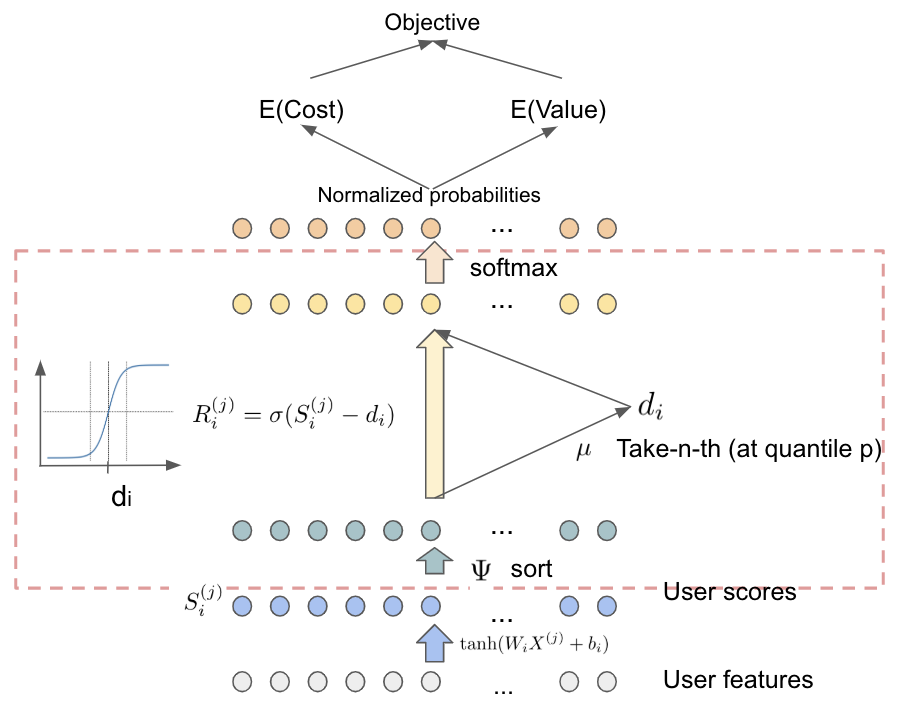
\includegraphics[width=\linewidth]{figures/fqr_figure}
  \caption{Illustration of the Fixed-Quantile-Ranking algorithm.}
\end{figure} 

\subsection{Sequential Causal Model with Deep Learning} 
It can be important to cadence of experimentation when we consider giving cohorts of users treatment. For instance, when a user was treated last week, what's the reaction to this week's treatment, or when users are treated frequently, there may be negative effects. In this section, we describe a causal learning algorithm with which we could learn the short-term and long-term correlations across time. To do so we perform causal learning on a sampler or ranker which takes temporal sequences into account. Concretely, we apply recurrent neural networks to model short term and long term states of users. The input to this system is a feature vector for a user at any given week. This feature vector contains information such as aggregated rides, average estimated time of arrival and other common characterizations of the user. The feature vector of any given user is time dependent and changes across weeks. 

\begin{figure}[h]
\label{seq_fig1}
  \centering
  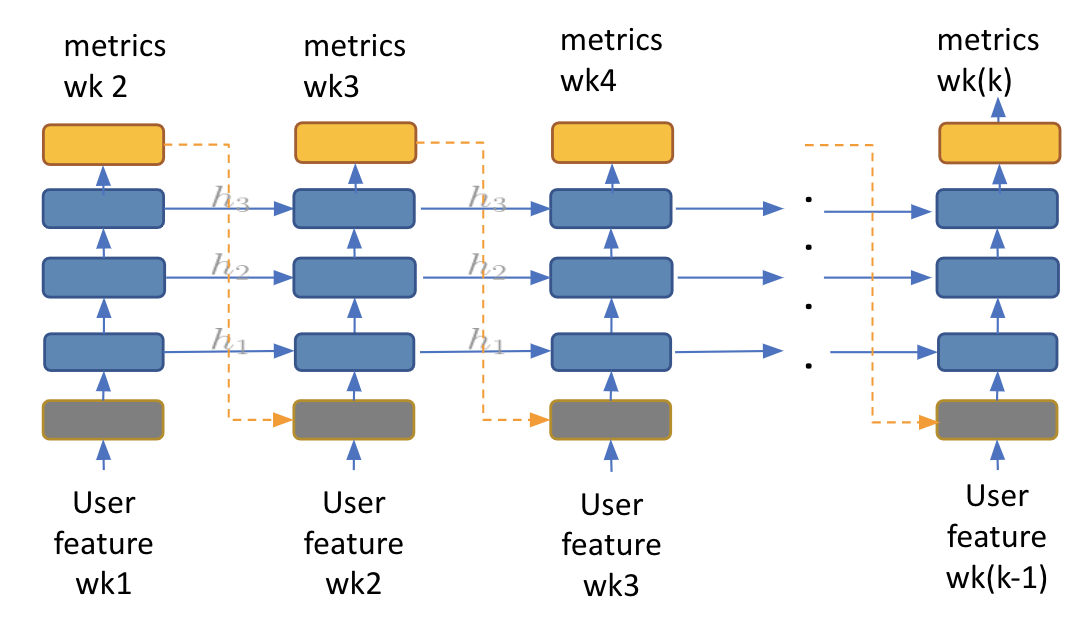
\includegraphics[width=\linewidth]{figures/seq_fig1}
  \caption{Formulation to represent users with sequential states.}
\end{figure} 

In order to construct an architecture that systematically correlates the sequence of states, and take into account the recurrent treatment labels, we resort to deep learning methods. First, the optimization objective in the previous section is abstracted into an epitomic module illustrated in Figure~\ref{drm_modular}. In this illustration, the operations to obtain ranker scores, separate cohorts, normalize and compute eventual objective is summarized into a module which takes in treatment and other metric labels, as well as ranker/sampler model score. 

\begin{figure}[h]
\label{drm_modular}
  \centering
  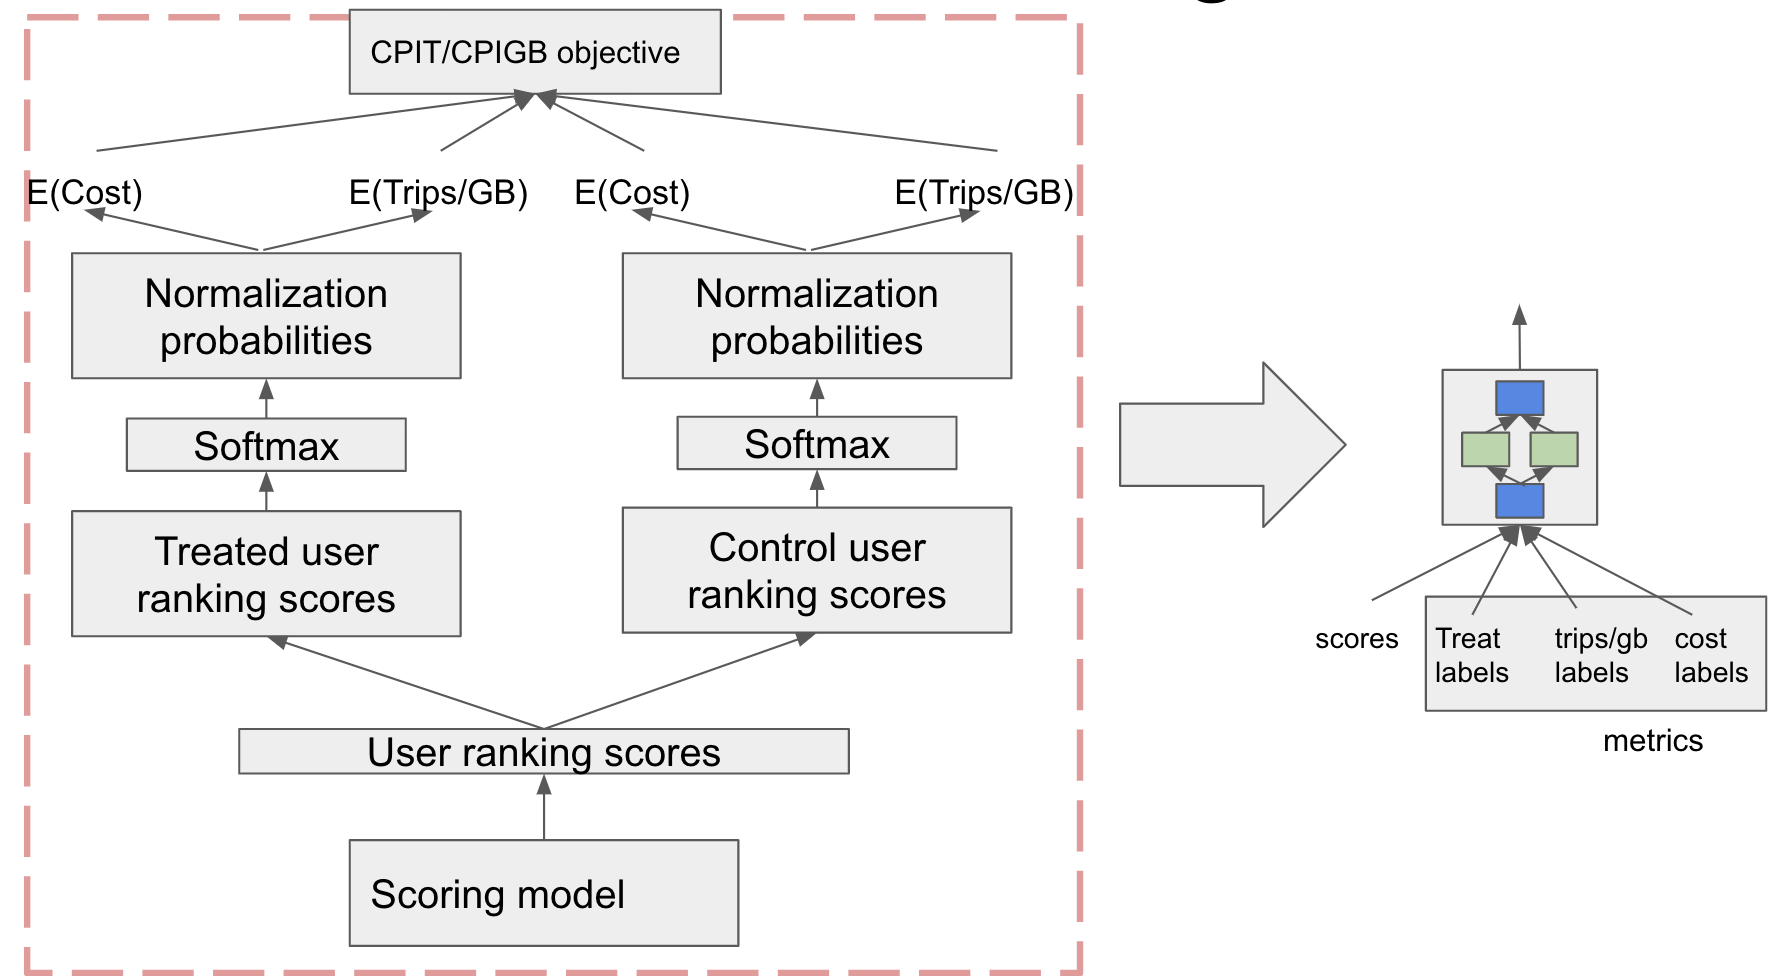
\includegraphics[width=\linewidth]{figures/drm_modular}
  \caption{Optimization objective function modularized to take in metrics and sampler/ranker score.}
\end{figure} 

Next, we combine this module with recurrent networks to obtain a deep learning architecture which models the changes in user states across multiple stacked layers, and correlates with the experimental metrics. Concretely, instead of being a simple regressor, the sampler/ranker is now a recurrent network with recurrent connections across time, this allows states in the past to influence the future, while able to score users at any given time step. Also, the optimization objective is computed and measured at each time step. During optimization, we are able to combine the errors from objective at all time-steps to optimize the recurrent sampler.  

In this recurrent model, we not only consider the user inputs at this time step, but also the metric outputs of the previous time step, this is analogous to the architecture of sequence to sequence models [ref needed]. Further the sampler or sampler of this model is simply the LSTM network. After the model is trained, we are able to score users at any given time in the past, so can use the last step thought vectors to evaluate the users at current time step. 

\begin{figure}[h] 
\label{seq_fig2} 
  \centering 
  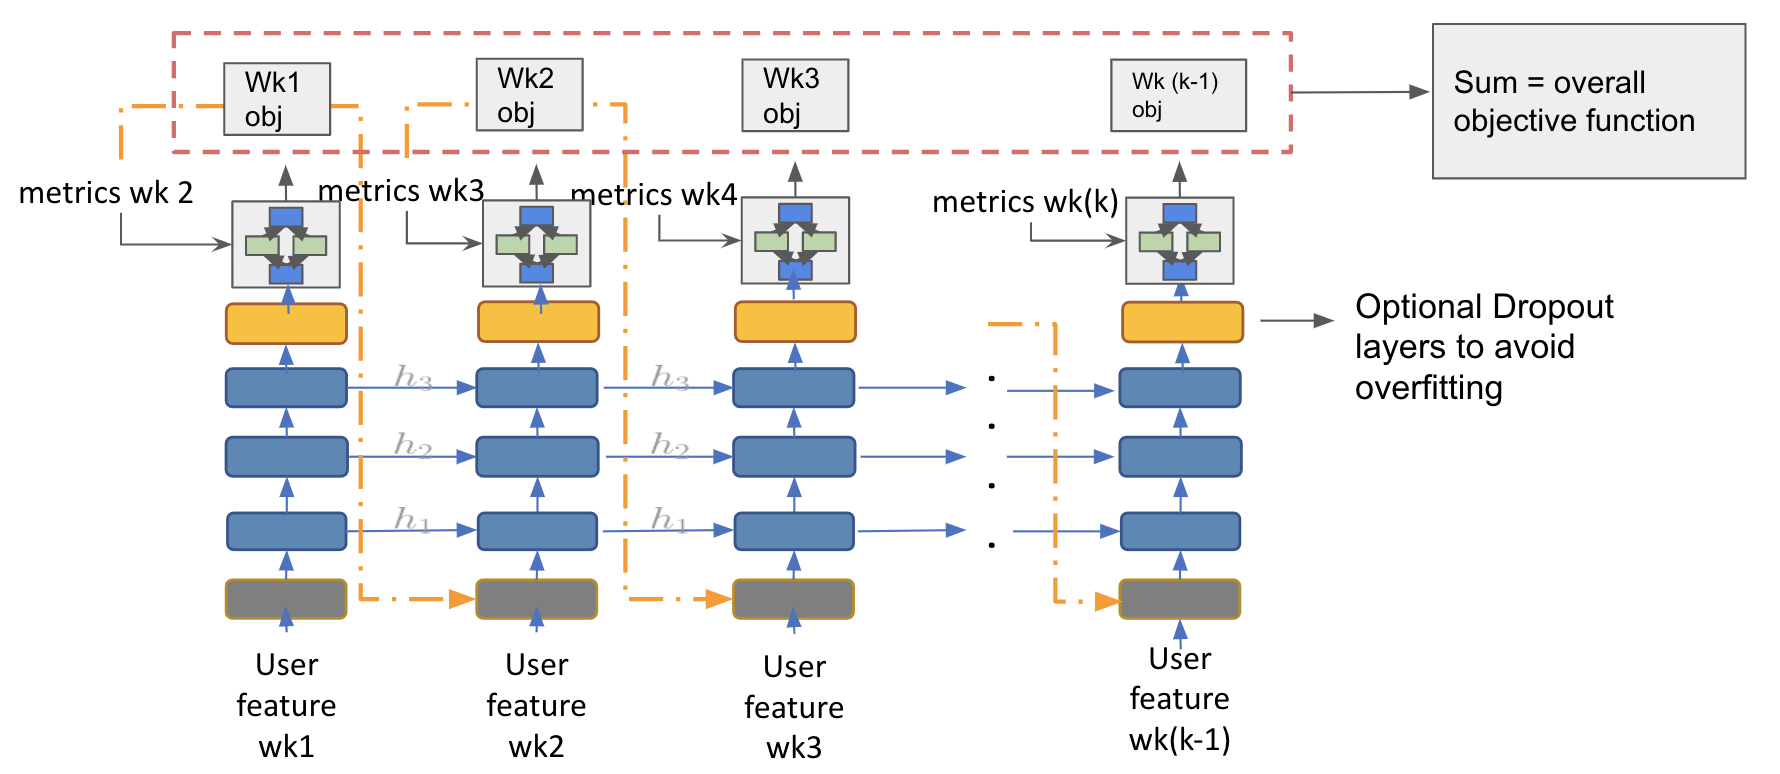
\includegraphics[width=\linewidth]{figures/seq_fig2} 
  \caption{Optimization objective function modularized to take in metrics and sampler/ranker score.} 
\end{figure} 

\subsection{Evaluation Methodology} 

The business objective is to achieve most incremental user retention with a given promotion cost budget. The retention and cost here are 2 critical values mentioned above for the causal ratio. 

\emph{Cost Curve}. Now that we have 2 treatment outcome $\tau^{retention}$ and $\tau^{cost}$ we care about, we draw a curve and use cost as X-axis and retention as Y-axis as the illustration below. 

\begin{figure}[h] 
\label{cost_curve_illustration} 
  \centering 
  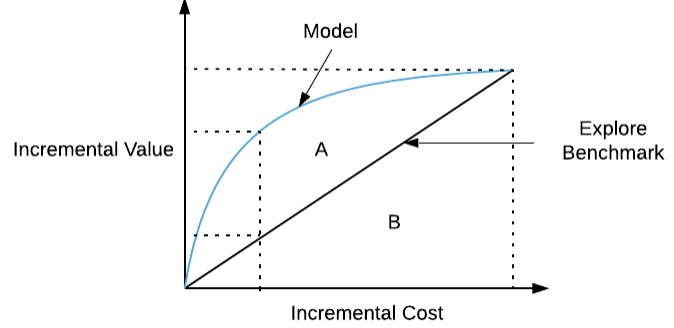
\includegraphics[width=\linewidth]{figures/cost_curve_illustration} 
  %\caption{Illustration of the Cost-Curve.} 
\end{figure} 

Similar to uplift curve, assume we have a score for each sample $S_i = f(X_i)$ that represents how good the sample is regarding the incremental cost and value. If we order samples by this score, then each point on the curve could be calculated from the $p$ percent highest scored samples, by taking the number of treatment samples times ATE (Average Treatment Effect) of this group. $\{W_i = 1 | S_i > S_i^{pth}\} \times ATE(x_i | S_i > S_i^{pth}) $ Note we can score the samples for both treatment and control as $f$ doesn’t depend on $W$. Here the function $f$ is the one we want to learn and we will discuss it in more details in the following section. 

Returning to the cost curve, as you increase the percent $p$ of samples to be included for each point, the aggregated incremental cost and value would increase (since you include more samples). So the end point of the cost curve (top right) is the one that includes all samples. And the origin (down left) is the one includes no sample. 

If the score $S_i$ is randomly generated, then there would be no difference between high and low score points regarding the ratio of incremental cost and value, and thus the cost curve should be a straight line. But if the score is generated by a good model, then the curve should be above the benchmark line. This means for the same level of incremental cost, a better model would select samples to achieve higher incremental value. 

Area Under Cost Curve (AUCC). Similar to Area Under Uplift Curve and AUC of ROC curve, here we use the area under cost curve as the numerical metric. To normalize the value, we use the ratio A/B as the AUCC, A and B are the area shown in the cost curve figure. A is the area between model curve and the benchmark curve, and B is the area under benchmark curve. The equivalent formula for AUC of ROC curve is (A+B)/2B = A/2B + 0.5 where A/B is the value that matters. The theoretical upper bound of A is B (the symmetric upper triangle), which means with no incremental cost we can achieve all incremental value from the sample. So this A/B should be bounded within [0, 1) and larger the AUCC, generally better the model.

\section{Empirical Results} 
\label{sec:empirical_results}
In this section, we will cover the empirical results for approaches (Causal Forest, R-Learner, DRM) mentioned above. The results include both offline out-of-sample test and online real-world launch. We will first describe the experiment data set and offline test setup. Then we would analyze both offline test results and real-world performance. In summary, cost curve offline evaluation is consistent with real-world result and DRM has the best performance. 

\subsection{Experiments} 
We launched a fully randomized explore experiment to collect data for model training and offline evaluation. 

We use a user level A/B test as the general framework. We generated a random uniformly distributed score and checked whether it’s above the threshold. If it was, we say it has been targeted and the sample would be censored and logged in our experiment. If not, we just ignore that sample. Each user will be only censored once for us to capture the long term effect. For targeted sample, we finally checked whether the user was in treatment or control cohort (A/B), only targeted sample in treatment got the promotion. This promotion was valid for one trip and expired in 7 days. 

The experiment period is 1 week where each user will get at most one promo. After the experiment week, we also have 4 blackout weeks that users who were censored during the experiment week will not get any other promotion during these blackout weeks. This helps us get the clean 4 week retention and cost outcome $Y^r$, $Y^c$.

\emph{Data}. In this experiment we collected over 1M trip (user) level data. The following table is an example of the data set we have. 

\begin{figure}[h] 
\label{feature_table} 
  \centering 
  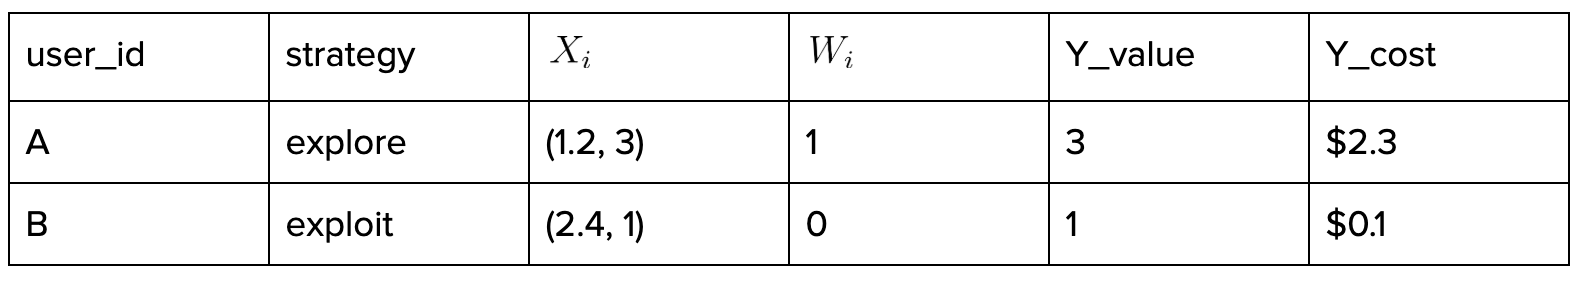
\includegraphics[width=\linewidth]{figures/feature_table} 
  %\caption{.} 
\end{figure} 

Features. Features are the key to estimate heterogeneous treatment effect. We use real-time trip features, time and geo features and user historical features for our modeling. 

We mainly use forward test in our evaluation. Specifically we split the data set into 3 parts: train, validation and test sets with 50\%, 20\%, 30\%. We first use the train and validation set to do the hyper-parameter optimization for each type of model. Once the hyper-parameter is finalized and fixed, we retrain the model on the train and validation set, and test it on the test set. 30\% might seem a high percentage for test split, this is due to the noisiness of treatment effect evaluation. In order to have a stable test evaluation, the test set should be large enough. 

In addition to forward test, we also did cross-validation test. Note, due to the heavy computation for hyper-parameter optimization, we still use the fixed hyper-parameter set we got above. Then we use 5-fold cross-validation on the whole data set for test evaluation. The results from cross-validation is consistent with the forward test. Since there might be some information leak between hyper-parameter optimization and cross-validation test, we only include the forward test results in the following section.

Details of the model structure are as follow.

R-Learner. We use Ridge Regression as the base estimator. Since we have fully randomized experiment, we use the constant treatment percentage as our propensity for all observations in the algorithm. Based on R-Learner original paper, Lasso and Boosting based method have similar performance, and currently we only have Ridge based algorithm implemented. As a next step, we are working on the implementation for Boosting and will include the results in future research. Lagrangian approach is used here. 

The iterative process to solve $\lambda$ could be slow as the value function $g$ here is piece-wise linear w.r.t $\lambda$. We take the approach to treat $\lambda$ as a hyper-parameter and determine its value through hyper-parameter optimization. 

Causal Forest. We use a random forest of causal trees, with 90 trees, 1000 as the minimum leaf size and 0.8 as the split alpha for scale between treatment effect and variance. Other hyper-parameters are not sensitive so we leave them as default values. Lagrangian approach is used here.

DRM. We have tried linear form and multiple different Multi Layer Perceptron (MLP) neural network structures. With the current non-sparse feature set, linear form has the best performance, so we use the linear form in this evaluation. We also include both L1 and L2 penalty with 0.1 as the scale factor. 

\subsection{Results} 
\subsubsection{Direct Ranking Model} 
Following are the cost curve on test set and the AUCC for each model. DRM is 5\% better than Causal Forest and 10\% better than R-Learner. All models are significantly better than the benchmark explore. One motivating example is to look at the vertical dash line at $\frac{1}{5}$ of total incremental cost, we can achieve 4X more incremental retention than random targeting by using the model here. 

\begin{figure}[h] 
\label{drm_result_curves} 
  \centering 
  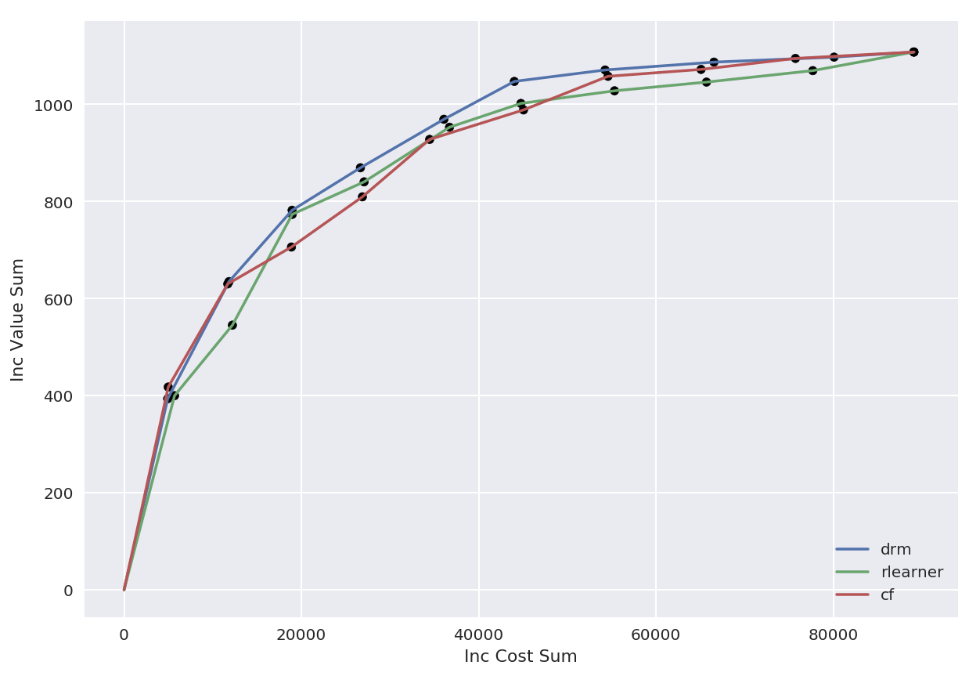
\includegraphics[width=\linewidth]{figures/drm_result_curves} 
  %\caption{Cost-Curve results for DRM vs rlearner vs causal forest model.} 
\end{figure} 

\begin{figure}[h] 
\label{drm_result_table} 
  \centering 
  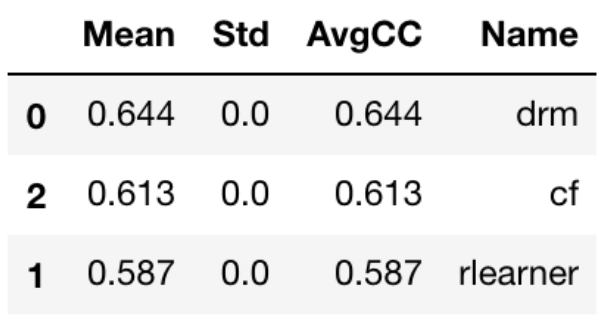
\includegraphics[width=0.4\linewidth]{figures/drm_result_table} 
  \caption{Cost-Curve results for DRM vs rlearner vs causal forest model.} 
\end{figure} 

\subsubsection{Top Quantile Ranking} 
We perform experiments with user incentives experiments given randomly in one city. The dataset contains 100,000 data points, and we split the dataset with 50\% training, 15\% validation and 35\% for testing. The model is trained on top quantile = 30\% and we evaluate the model with efficiency at this fixed quantile on the cost-curve. As shown in Figure below, the efficiency can be improved significantly using top quantile ranking method. 

\begin{figure}[h] 
\label{fqr_results_compare} 
  \centering 
  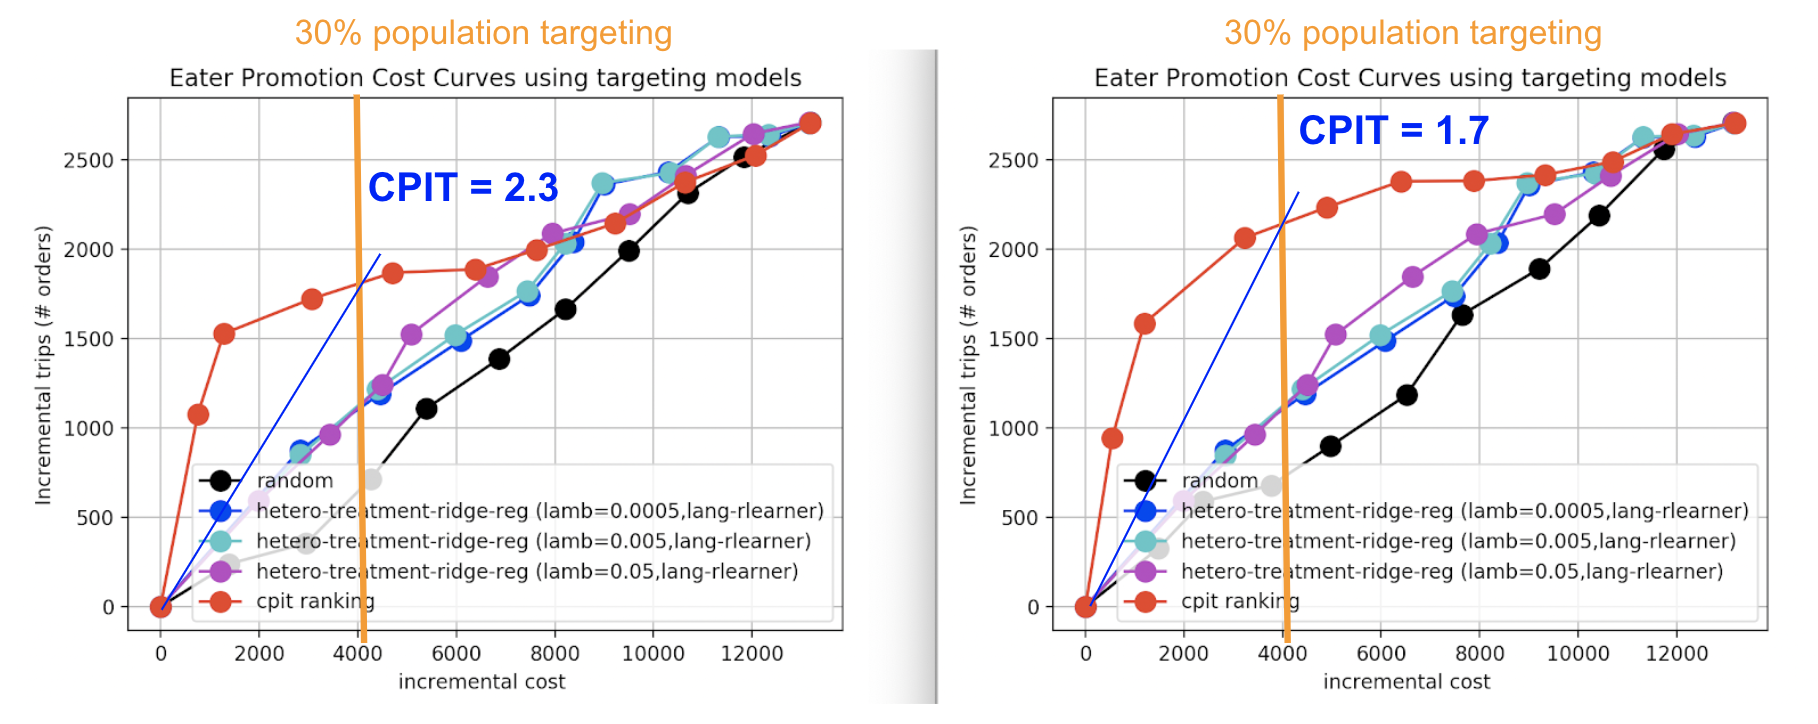
\includegraphics[width=\linewidth]{figures/fqr_results_compare} 
  \caption{Cost-Curve results for top quantile ranking model.} 
\end{figure} 

\subsubsection{Sequential Causal Learning Model} 
We evaluate our model built with sequential user states using sequential experimental data. 

\textbf{Model and training} In our implementation, we use Tensorflow framework (v2.0) using the \emph{dynamic\_rnn} api to implement recurrent neural networks. Specifically, we implement at multi-layer stacked LSTM as the recurrent sampler. 

To speed-up the process, we use a minibatching algorithm for optimization. To minibatch the objective function introduced in previous section is not difficult. We simply take a larger minibatch where each cohort have significant number of users. In practice, the minibatch size is taken to be around 10,000. This is sufficient to obtain high-quality gradients. The model is optimized with Adam optimizer with learning rate of 0.01 and $\beta_1 = 0.5, \beta_2 = 0.999$. To avoid gradient explosion problems, we train the model using $L2$ gradient clipping at threshold of $2.3$. 

\textbf{Data prepration} We extracted data from 21 larger US cities and data is extracted on a weekly cadence for a total of 11 weeks. This results in 1.2 million distinct users and 2.4 million records from logs. We split the data into training, validation and testing, resulting in 1.3 treatment instances aggregated across time, and 330,000 control instances. The data has bias to treatment due to emphasis on results in production. We combine treatment with small differences to increase the density of data across time and mitigate sequence sparsity. 

There is a portion of sequential data that is missing in the logging system. For instance, user A was treated in week1, not tracked in weeks 2,3 and was in control group in week4. To deal with missing data, we use two techniques. First, we would mask training and evaluation processes only with existent data. For instance when training, only errors from objective function where sequential data exists is taken into account during model learning. For evaluation, the metrics are computed without missing data. When data is missing at any time step, we use a zero user feature vector as input to the model. This removes any influence to the recurrent computation of the LSTMs. 

\textbf{Results of sequential causal model} The sequential model is evaluated across multiple architectures, and the results in the below table and figure show they are significantly better than the previous method without sequential information. 

\begin{table}
  \caption{Results of the sequential causal model.}
  \label{res}
  \begin{tabular}{lllll}
    \toprule
    Architecture&HSCL&. &Baseline& \\
    \midrule
    num units & TrCPIT & TePIT &TrCPIT & TeCPIT\\ 
    \midrule 
    1 layer LSTM $[6]$ & 7.17 & 7.80 & 8.01& 10.00 \\
    1 layer LSTM $[16]$ & 6.89 & 8.35 & 7.69& 8.93 \\
    2 layer LSTM $[16, 16]$ & 5.90 & 6.97 & 8.39& 9.65 \\
    3 layer LSTM $[8, 8, 8]$ & 7.35 & 8.64 & 7.97 & 9.73 \\
    \bottomrule
\end{tabular}
\end{table}

\begin{figure}[h] 
\label{hscl_results} 
  \centering 
  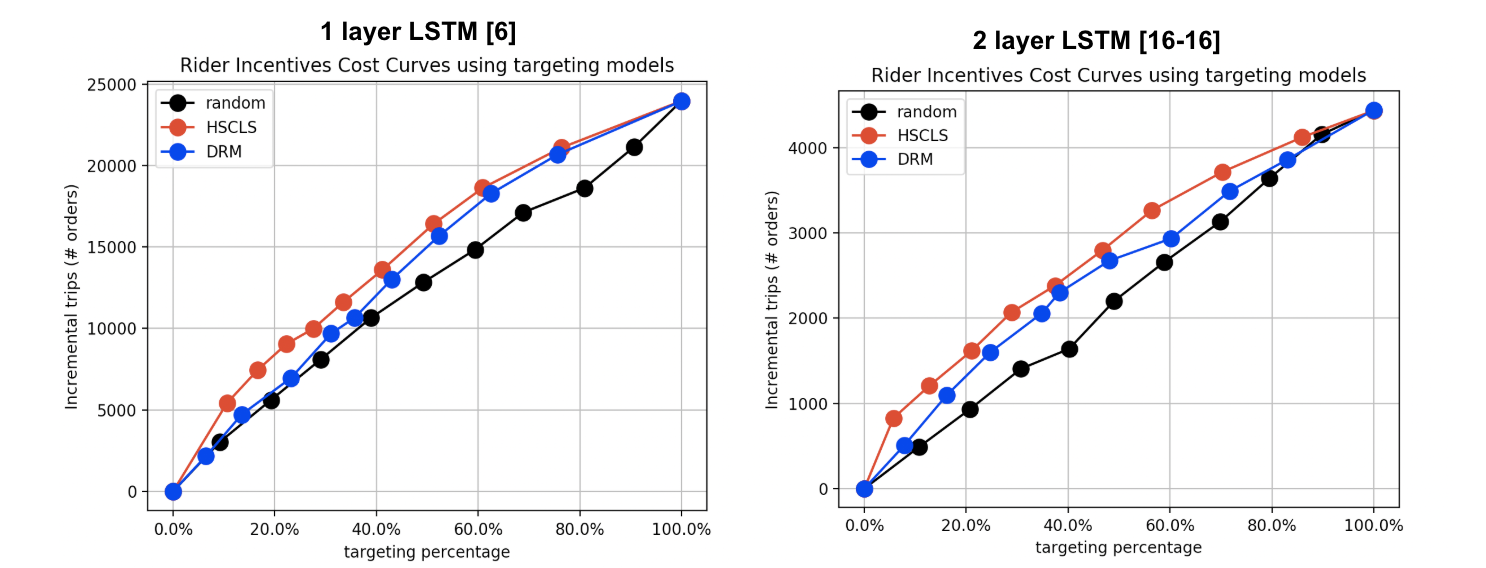
\includegraphics[width=\linewidth]{figures/hscl_results} 
  \caption{Cost-Curve results for sequential causal learning model on the held-out test set.} 
\end{figure} 

\section{Conclusion and Future Work} 

\subsection{Conclusion} 
We propose a novel ranking method to optimize heterogeneous promotion treatment effect for user retention. The method combines prediction and optimization into one single stage and provides a general loss function that can be incorporated with any differentiable functional form including linear and neural network structure. We also provide an empirical evaluation metric and adjustments for existing estimator for the promotion treatment effect optimization problem. We evaluate various methods empirically both offline and online. Our proposed method achieves significantly better performance than explore benchmark and existing estimators. After successful test, this method has been deployed to production and is live in many cities all over the world.

\subsection{Future Work} 
\emph{Smart Explore/Exploit}. In current work we use epsilon-greedy explore, where we split a fixed percentage of budget to spend on fully randomized explore to collect data for model training. However, this will sacrifice the performance and is suboptimal. As a better approach, we will try to use multi-arm bandit or Bayesian optimization framework to guide our smart explore based on the model uncertainty. 

\emph{Deep Embedding}. Raw time and geo features are extremely sparse. Various embedding techniques have been used for sparse features but none of them is specifically for treatment effect. As treatment effect is different from its underlying outcome, the embedding should also be different. Now that we have a general loss function which could be incorporated with any neural network structure, we could start to work on the embeddings specifically for treatment effects. 

%From the table below we can observe a consistent improvement (the lower the better) with using the sequential causal learning system. 

%%
%% The next two lines define the bibliography style to be used, and
%% the bibliography file.
\bibliographystyle{ACM-Reference-Format}
\bibliography{references}

\end{document} 

%\endinput 
%% 
%% End of file `sample-authordraft.tex'. 
